\documentclass[11pt]{article}
\usepackage{amsmath,amsthm,amssymb,wasysym}
\usepackage{mathtools}
\usepackage{enumerate}
\usepackage{graphicx}
\usepackage{mathpazo}
\usepackage{lmodern}
\usepackage{parskip}
\usepackage{fancyhdr}
\usepackage{wrapfig}
\usepackage{tikz}
\usepackage{hyperref}
\usepackage{listings}
\lstset
{
    language=Python,
    basicstyle=\footnotesize,
    numbers=left,
    stepnumber=1,
    showstringspaces=false,
    tabsize=1,
    breaklines=true,
    breakatwhitespace=false,
}
\usepackage[linesnumbered,algoruled,boxed,lined]{algorithm2e}
\usetikzlibrary{positioning, shapes.geometric, arrows}
\tikzstyle{startstop} = [rectangle, rounded corners, text centered, draw=black, fill=red!30]
\tikzstyle{io} = [text centered]
\tikzstyle{decision} = [rectangle, text centered, draw=black]
\tikzstyle{process} = [trapezium, text centered, draw=black]
\tikzstyle{arrow} = [thick,->,>=stealth]
\newtheorem{theorem}{Theorem}
\newtheorem{defn}{Definition}
\newcommand{\Jostle}{\texttt{Jostle}}
\lhead{Senior Thesis}
\rhead{Jacob Imola}
\cfoot{\thepage}
\pagestyle{fancy}
\title{Automatic, Fine-Grained Algorithmic Choice for Differential Privacy}
\date{\today}
\author{Jacob Imola\\ School of Computer Science, Carnegie Mellon University\and Jean Yang\\ School of Computer Science, Carnegie Mellon University}
\begin{document}
\maketitle
\section{Introduction}
The rapid technological increase in data collection, speed, and storage has brought about revolutionary insights and ideas and will continue to do so. However, with huge amounts of private data comes the concern of preventing data from ending up in the wrong hands. In order to prevent data leakage, we must lay a strong privacy foundation and give data analysts the tools for them to implement privacy efficiently and correctly.

Consider a healthcare database with records like patient weight, age, some genetic information, or whether they are HIV positive. Granting access rights, or policies, to just patients and their doctors protects as much privacy as possible, and developing tools for verifying information flow policies is an interesting question in its own right. However, sometimes it's okay to release a few general statistics about a database so that an analyst can find risk factors for people who have HIV. On the other side of the spectrum, publicly releasing the entire database doesn't protect privacy at all, yet it would be an analyst's dream. In order to appease both data analysts and patients, a middle ground area must be chosen where a blurry snapshot of the database is released, comprehensive enough so that meaningful conclusions may be drawn yet blurry enough so that individuals are mostly protected. We call this the \emph{privacy-accuracy} tradeoff. We can always sacrifice one for the other before we disclose our database snapshot. However, after we disclose, it is impossible to take any privacy back, so we have to be absolutely sure that privacy guarantee will not fail under any attack. The most promising method for doing such a disclosure is Differential Privacy \cite{Dwork:2006}.

Differential Privacy (DP) is considered to be the gold-standard of privacy and has been researched intensely since its conception in 2005. Its goal is to provide guarantees on what can be done with the information being released from a dataset making minimal assumptions about an attacker's powers. Previous attempts were not mathematically rigorous and did not reliably prevent attacks. Notably, before DP, researchers were able to reidentify users in a Netflix dataset given an auxiliary dataset from IMDB and form a generalized attack against the state-of-the-art privacy algorithms of the time \cite{Narayanan:2006}. The strong privacy guarantee of DP, on the other hand, has a rigorous mathematical foundation that makes it impervious to the post-processing attacks that exploited the Netflix dataset, and more recently, \href{https://hackernoon.com/how-to-rob-an-airbnb-252e7e7eda44}{AirBnB} and \href{https://gizmodo.com/this-is-almost-certainly-james-comey-s-twitter-account-1793843641}{Instagram}. Differential Privacy has certainly stood the test of time as a sturdy way to protect privacy.

However, just building a suite of DP algorithms is not satisfactory. Privacy adds a new layer of complexity to the data analyst's job because the performance of algorithms may vary wildly depending on the database or on other parameters, complexity that an analyst may not fully understand. Most data analysts are not Differential Privacy experts. This leads to the central problem of this work: 

\textbf{Problem:} How can we help data analysts dispatch Differential Privacy algorithms in a way that helps them understand the privacy and accuracy tradeoff space?

This problem is noted by the authors of DPComp \cite{Hay:2016}, who comment that currently, ``the practitioner is lost and incapable of deploying the right algorithm''. DPComp allows the analyst to visualize the performances of different histogram querying algorithms on certain datasets. An example dataset  is shown in Figure \ref{fig:dpcomp}. We feel this is a step in the right direction, but there are two main drawbacks: their visualization tools are limited to 2D histogram algorithms, and they don't help the programmer enough on his actual dataset, instead using publicly available knowledge. To address both of these issues, we take a programming-language-based approach. The approach is to move the manual exploration of algorithms that an analyst might do with DPComp into the runtime of our programming language, which we call \Jostle{}. This will preserve the insights that an analyst may gleam from DPComp (since the algorithmic choice will be publicly available to him) and will confer the advantages of a programming language:

\begin{figure}
\begin{center}
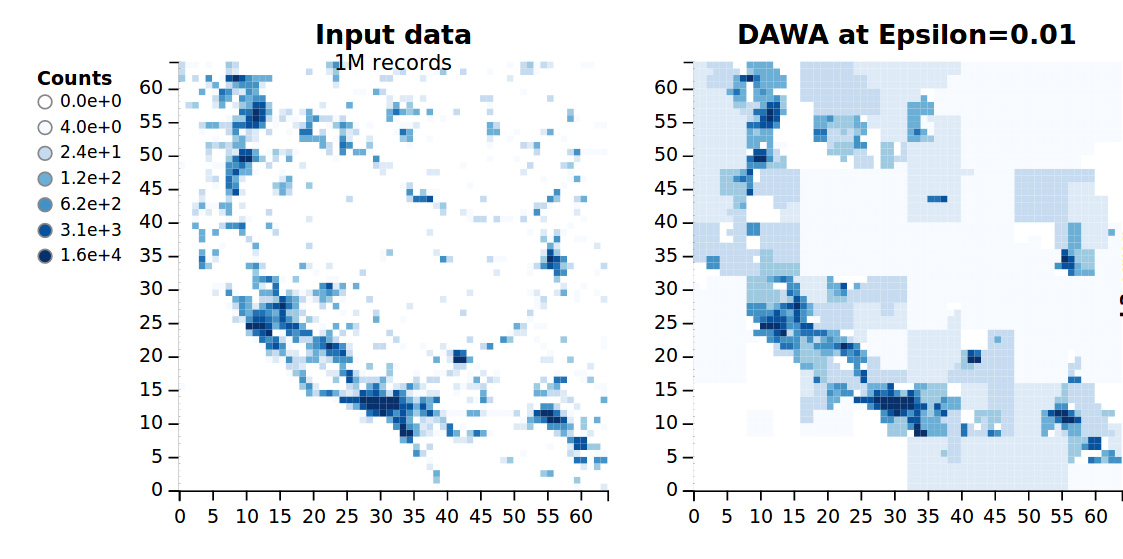
\includegraphics[scale=0.3]{DPComp}
\end{center}
\caption{A screenshot of a DPComp graph depicting the original dataset and the noise that a DP algorthm, DAWA \cite{Li:2014}, adds at $\epsilon=0.01$. This would help an analyst decide whether to apply DAWA on his own dataset.}\label{fig:dpcomp}
\end{figure}
\begin{itemize}
\item \textbf{Abstraction} Creating an abstraction for algorithmic choice in a programming language allows for the suppression of complicated privacy machinery, allowing analysts to view the choice as a black box. In fact, a programmer could view all of DP as a black box and still use \Jostle{} by simply trying many DP black boxes and knowing that the best algorithm will be used \footnote{We could call these programmers privacy-agnostic.}. Programmers write code faster with fewer bugs when they can think about complicated ideas as black boxes.
\item \textbf{Generalization} As previously noted, it is infeasible to conduct experiments like DPComp on all use cases that an analyst may encounter. Writing a sophisticated programming language that automatically makes this choice would eliminate the need for this while still allowing for high-grade code performing as if the experiments had been conducted.
\end{itemize}

The most central idea in \Jostle{} is the \texttt{NoisyIf} statement, illustrated in Figure \ref{fig:1}.
\begin{figure}
\begin{lstlisting}
def f(D):
    NoisyIf(g D):
        do A
    else:
        do B
\end{lstlisting}
\caption{Example \texttt{NoisyIf} statement.}
\label{fig:1}
\end{figure}
A programmer will use \texttt{NoisyIf} when they are unsure of which choice to make at a certain point in their code. If they have certain beliefs that may aid \Jostle{} in making the choice, then they may specify an \emph{advice} function (denoted by \texttt{g} in Figure \ref{fig:1}). Jostle will combine this advice along with previous executions of this particular \texttt{NoisyIf} to make the best decision.

We will begin with a background section on DP and related work. Then we will introduce decision trees and highlight the existence of Problem with them. Thirdly, we will solve the decision tree problem with different \texttt{NoisyIf} statements, and finally, we will illustrate how \texttt{NoisyIf} statements can be generalized to make \texttt{Jostle}.

\section{Background}
\subsection{Differential Privacy}
DP is motivated by the example of a subject being asked to participate in a study involving an algorithm $\mathcal{A}$ being run on a database $D$. If $\mathcal{A}(D)$ changes as a result of the subject participating, then this poses a privacy concern. An attacker may be able to infer something about the participant's input. This means that non-trivial deterministic algorithms are already unacceptable; their output may change depending on just a single addition to $D$. The strength $\epsilon$ of a DP guarantee is the maximum factor that the randomized output of $\mathcal{A}$ changes for two databases $D$ and $D'$ which differ in one row. Mathematically, we are saying:

\begin{defn}
$\mathcal{A}$ satisfies $\epsilon$-DP if for all $D$ and $D'$ such that $|D-D'|_1=1$ and for all $o$ in the range of $\mathcal{A}$, 
\[\Pr\left(\mathcal{A}(D) = o \right) \leq e^{\epsilon} \Pr\left(\mathcal{A}(D')=o\right)\]
\end{defn}

There is also a weaker definition: 

\begin{defn}
$\mathcal{A}$ satisfies $(\epsilon, \delta)$-DP if for all $D$ and $D'$ such that $|D-D'|_1=1$ and for all $o$ in the range of $\mathcal{A}$, 
\[\Pr\left(\mathcal{A}(D) = o \right) \leq e^{\epsilon} \Pr\left(\mathcal{A}(D')=o \right) + \delta\]
\end{defn}

For much of this paper, we will focus on $\epsilon$-DP, but it is worth knowing the more general case so we can import the well-known privacy theorems in their most general form. Below is perhaps the most important result, and its proof comes cleanly from the definition of DP.

\begin{theorem}
(Post-Processing \cite{Dwork:2006}) If $\mathcal{A}$ satisfies $(\epsilon, \delta)$-DP, and $F$ is any function that takes the output of $\mathcal{A}$ as input, then $F(\mathcal{A})$ satisfies $(\epsilon, \delta)$-DP.
\end{theorem}
This theorem is the reason why DP is such a useful guarantee. Data analysts can be sure that once they run their algorithm $\mathcal{A}$ and release its output, then the DP guarantee gets no weaker \emph{no matter what an adversary does with the data}. This prevents the headaches where an analyst realizes retroactively that the data he released can be combined in some way to reveal much more information than was intended. Another useful, intuitive result is:

\begin{theorem} \label{thm:comp}
(Composition \cite{Dwork:2006}) Given algorithms $M_1$ and $M_2$ satisfying $\epsilon_1$ and $\epsilon_2$ DP, respectively, along with a database $D$, the algorithm $M = (M_1(D), M_2(D))$ has $(\epsilon_1+\epsilon_2, \delta_1+\delta_2)$ DP.
\end{theorem}
Composition is like the union bound from probability; it's convenient to apply but often is a pessimistic bound, as we will see later. Because of composition, we often refer to $\epsilon$ as a privacy budget---if we string together many private computations, it's like we spend some of our budget on them, and our total budget is $\epsilon$.

Finally, we can talk about the disjointness of our queries---if $D$ is split into disjoint parts, before mechanisms are applied to it, then out of all its possible neighbors, only one of the parts will be different. Thus, only the worst mechanism will affect the guarantee:
\begin{theorem}\label{thm:disj}
(Disjointness \cite{Dwork:2006}) Given disjoint subsets $D_1, D_2$ of $D$ with two mechanisms $M_1$ and $M_2$ providing $(\epsilon_1, \delta_1)$ and $(\epsilon_2, \delta_2)$-privacy, then $((M_1(D_1), M_2(D_2))$ satisfies $(\max\{\epsilon_1, \epsilon_2\}, \max\{\delta_1, \delta_2\})$-DP.
\end{theorem}

So, what's a simple example of a DP algorithm? Suppose each row of our database $D$ is 0 or 1, so $D \in \{0, 1\}^n$, and that we are trying to release the sum of the elements of $D$. If this sum is $S$, then all neighboring databases $D'$ have sum $S$ or $S+1$. We can add noise to $S$ so that it looks very similar in distribution to $S+1$. The distribution we are looking for is the Laplace distribution:
\begin{defn}
The $\text{Laplace}(\lambda)$ distribution has probability mass function $f(x) = \frac{1}{2\lambda}e^{-|x|/\lambda}$.
\end{defn}
This distribution fits perfectly with the definition of DP because of the exponentials. If $X,Y$ are i.i.d. from $\text{Laplace}\left(\frac{1}{\epsilon}\right)$, then it is straightforward to show that the distributions of $S+X$ and $S+1+X$ satisfy $(\epsilon, 0)$ DP. To generalize this statement, we will use the following definition:
\begin{defn}
(Sensitivity) A function $f$ is $\Delta$-sensitive if for all $x,y$ such that $|x-y|_1 = 1$, we have 
\[
|f(x) - f(y)| \leq \Delta
\]
This can equivalently be rephrased as 
\[
\max_{|x-y|_1=1}|f(x) - f(y)| = \Delta
\]
We will denote the sensitivity of $f$ by $\Delta(f)$.
\end{defn}
This gives us the following mechanism:

\begin{algorithm}\label{alg:1}
\SetAlgoLined
\SetKwInOut{Input}{Input}\SetKwInOut{Output}{Output}
\Input{$D$, a database; $f$, a function $\mathcal{D} \rightarrow \mathbb{R}^n$; and $\epsilon$}
\Output{An estimate for $f(D)$ satisfying $\epsilon$-DP.}
$X$, a vector of $n$ i.i.d. variables drawn from $\text{Laplace}\left(\frac{\Delta(f)}{\epsilon}\right)$\;
\Return{X+f(D)}
\caption{Laplace Mechanism}
\end{algorithm}

\begin{theorem}
The Laplace Mechanism \ref{alg:1} satisfies $(\epsilon, 0)$-DP \cite{Dwork:2006}.
\end{theorem}
For the counting or histogram queries such as our example above, we have $\Delta = 1$ so we add $\text{Laplace}\left(\frac{1}{\epsilon}\right)$ noise to our function.

However, what if we wanted to compute the maximum value in a set? If we had $n$ elements, we certainly wouldn't want to apply Composition $n$ times, obtaining $n\epsilon$-DP, just to have $\texttt{Laplace}\left(\frac{1}{\epsilon}\right)$ noise added to our answer. A better way is to use ReportNoisyMax \ref{alg:max}. Instead of paying $n\epsilon$, ReportNoisyMax allows us to pay $\epsilon$ for the exact same noise on our answer.
\begin{algorithm}\label{alg:max}
\SetAlgoLined
\SetKwInOut{Input}{Input}\SetKwInOut{Output}{Output}
\Input{$D \in \mathcal{D}$, $\mathcal{X}$, a domain; $f$, a function $\mathcal{X} \times \mathcal{D} \rightarrow \mathbb{R}$; and $\epsilon$}
\Output{$x \in \mathcal{X}$ that attains maximum value on $f(S)$, satisfying $\epsilon$-DP.}
$X$, a vector of $|\mathcal{X}|$ i.i.d. variables drawn from $\text{Laplace}\left(\frac{\Delta(f)}{\epsilon}\right)$\;
\Return{$\arg\max_{i=1}^{|\mathcal{X}|}\{ X+f(\mathcal{X})\}$}
\caption{ReportNoisyMax}
\end{algorithm}
However, ReportNoisyMax only works on monotone queries, or where $f(x, D) < f(x, D')$ for all $x \in X'$. A version that works on queries in general is the Exponential Mechanism \ref{alg:exp}.
\begin{algorithm}\label{alg:exp}
\SetAlgoLined
\SetKwInOut{Input}{Input}\SetKwInOut{Output}{Output}
\Input{$D\in \mathcal{D}$; $\mathcal{X}$, a domain; $f : \mathcal{X}\times \mathcal{D} \rightarrow \mathbb{R}$, a utility function, $\epsilon$}
\Output{$x \in \mathcal{X}$ where $f(x, D)$ is more likely to be high.}
Pick $x \in \mathcal{X}$ where $\Pr(x=k) \propto \exp\left(\frac{\epsilon f(k, D)}{2\Delta(f)}\right)$\;
\Return{$x$}
\caption{Exponential Mechanism}
\end{algorithm}
ReportNoisyMax doesn't have a factor of 2 in its Laplacian noise, and this means a lighter tail. Thus, for monotone queries, we use ReportNoisyMax.
\subsection{Related Work}

Perhaps the best-known example of a language that attempts to help practitioners use DP is PINQ \cite{McSherry:2010}. PINQ builds off Microsoft's C-sharp LINQ database system and provides an interface between the database and the programmer that can accomplish simple differential-privacy mechanisms. PINQ makes extensive use of the Laplace Mechamism \ref{alg:1} to noise histogram queries such as \texttt{Count}, \texttt{Average}, and \texttt{Median}. It also uses Composition \ref{thm:comp} extensively when many of these queries are executed, and it attempts to abstract the composition into a \texttt{PINQAgent} class which keeps track of privacy budget. For example, the \texttt{NoisyCount} function is implemented in Figure \ref{fig:PINQNoisyCount}
\begin{figure}
\begin{verbatim}
double NoisyCount(double epsilon){
    if(myagent.apply(epsilon)){
        return mysource.Count() + Laplace(1.0/epsilon);
    }else{
        throw new Exception("Access Denied")
    }
}
\end{verbatim}
\caption{NoisyCount Implemented in PINQ.}
\label{fig:PINQNoisyCount}
\end{figure}
The amount of code that can be written in PINQ is surprisingly large; indeed, McSherry provides implementations of $k$-means and Social Networking. Also, the interface is a step in the right direction of thinking about privacy as a black box. However, the drawback of PINQ is that an analyst must still think about noise at every step of the computation. If an \texttt{Access is denied} error is thrown or the results are unacceptably noisy, the analyst will have no idea how to fix their code without diving into privacy.

Several languages have been built off PINQ to try to increase its functionality \cite{Proserpio:2014} \cite{Johnson:2017}. wPINQ \cite{Proserpio:2014} uses a weighted database which is a function $f : \mathcal{D}^n \rightarrow \mathbb{R}$, which can be thought of a generalization of regular databases where each element appears a natural number of times. Proserpio et al. define \texttt{Join} on two weighted databases in a way that greatly reduces the weights of elements that appear many times in the resulting join.

For instance, in a complete bipartite graph with $n$ vertices, there are no triangles. However, the addition of a single edge can add $O(n)$ triangles to the graph, so the triangle-counting function is very sensitive. If we were to count the number of triangles given a database $D$ of all the edges, we could start with the standard outer Join, $\texttt{Join}(D, D)$, to produce paths of length 2. Indeed, this produces a database where $O(n)$ elements could vary when a single edge is changed. To prevent this problem, the authors define a new type of Join, where the weight of an element in $\texttt{Join}(D, D)$ is inversely proportional to the number of times each vertex in the path appears in any path of length 2. This curbs the sensitivity immensely, and the authors succeed in counting the number of triangles (or any design) using their version of \texttt{Join}.

The authors of \cite{Johnson:2017} overcome the large sensitivity of \texttt{Join} by forcing the predicate of the Join to be just equality of keys. This greatly reduces the amount that a single record can change the result of \texttt{Join}.

In Fuzz \cite{Reed:2010}, a type system is implemented to guarantee differential privacy and sensitivity. Each type is endowed with a metric, and judgments are given for richer programming constructs such as sums, products, recursive types, and lambda expressions. Once the type of the program is known, its metric is known and its sensitivity can be inferred from the input variables. Sensitivity allows us to add the proper amount of noise via the Laplace Mechanism. To go from an $\epsilon$-sensitive function to an $\epsilon$-DP function, noise is added via a monad by applying the function $add\_noise : \mathbb{R} \multimap \fullmoon\mathbb{R}$.

For instance, counting the number of people in a database older than 40 could be achieved by:
\[
add\_noise\;(size\;(filter\;over_{40}\;db)) : db \multimap \fullmoon\mathbb{R}
\]

However, there are two shortcomings with this method. First, the analyst is still responsible for adding noise and making decisions that affect the sensitivity of a computation. Perhaps it's better to defer the adding of noise of the 
\subsection{Existing Methods for Algorithmic Choice}

Limited versions of algorithmic choice have been demonstrated in previous work. These methods focus on giving the analyst the ability to choose an $\epsilon$, evaluate whether the computations is satisfactory, and then have the option of increasing $\epsilon$ if the computation is deemed unsatisfactory.
For instance, if the analyst is training a private linear regression model that requires her to release $(X^TX)^{-1}X^Ty$ for a matrix $X$ and output vector $y$, then it's easy for her to compute the sensitivity of her function and apply the Laplace Mechanism to the output. However, it's not easy to know ex-ante exactly how high $\epsilon$ should be to result in a fit that has, for example, less than 5 mean square error.

This problem is addressed by Koufogiannis et. al \cite{Koufogiannis:2015} who give a general method for releasing any computation based on the Laplace Mechanism \emph{gradually}. In their version of the Laplace Mechanism, an analyst selects a set of increasing $\epsilon$ values, $(\epsilon_1, \epsilon_2, \ldots, \epsilon_T)$. Their main result is finding a way to generate Laplace variables $(v_1, v_2, \ldots, v_T)$ such that knowing a prefix $(v_1, v_2, \ldots, v_t)$ is $\epsilon_t$-DP and, with high probability, the noise generated by $v_i$ is no worse than the noise added by the standard Laplace Mechanism for guaranteeing $\epsilon_t$-differential privacy. They accomplish this by correlating the $v_i$'s in an intelligent way. Ligett et. al \cite{Ligett:2017} take this one step further by describing a way to iterate through the $v_i$'s until a suitably accurate algorithm is selected. Accuracy can be specified by the analyst as an arbitrary function that takes in a $v_i$. Of course, the release of the most-accurate mechanism has to be done in a differentially-private manner as well, and Ligett et. al use an adaptation of the AboveThreshold mechanism \cite{Dwork:2006}. This results in an additional privacy and accuracy penalty over simply using the Laplace Mechanism with a fixed $\epsilon$. Specifically, if $v_t$ is chosen, then the computation is $\epsilon_t+\epsilon_A$-DP.

We notice the following problems with the methods addressed above:
\begin{itemize}
\item AboveThreshold does not work on releasing $(\epsilon, \delta)$-DP mechanisms with $\delta > 0$.
\item A privacy and accuracy penalty is taken when selecting the best algorithm. This method is rather arbitrary; how do we select $\epsilon_A$? Is this even the optimal way of algorithm selection?
\item The papers only work on the specialized case of the Laplace Mechanism.

More papers to talk about: \cite{Winograd-Cort:2017}, \cite{Liu:2018}, \cite{Hsu:2014}.
\end{itemize}
\subsection{Decision Trees}

Decision Trees are a powerful tool for data mining due to their high human interpretability, non-parametric design, low computational cost, ability to discover non-linear relationships among attributes, resilience to missing values, ability to handle both discrete and continuous data, and ability to handle non-binary labels \cite{Fletcher:2016}. Let our database again be $D$, and suppose it has $k$ columns or attributes, the $i$th of which can take values in $\mathcal{A}_i$. Let $\mathcal{C}$ be the output attribute, or class, which we are trying to predict. We assume for simplicity that $\mathcal{A}_i$ and $\mathcal{C}$ are discrete sets. A decision tree classifies points by branching on attribute $\mathcal{A}_i$, forming $|\mathcal{A}_i|$ subtrees. Once certain criteria are met, no more branching occurs, and instead a leaf node predicts the class. An example Decision Tree is given in Figure \ref{fig:dt}.

\begin{figure}
\begin{center}
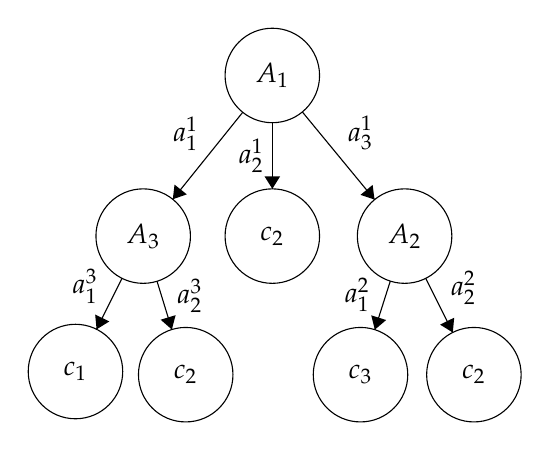
\begin{tikzpicture}[scale=0.2]
\tikzstyle{every node}+=[inner sep=0pt]
\draw [black] (18.1,-4.4) circle (3);
\draw (18.1,-4.4) node {$A_1$};
\draw [black] (9.9,-14.6) circle (3);
\draw (9.9,-14.6) node {$A_3$};
\draw [black] (5.6,-23.2) circle (3);
\draw (5.6,-23.2) node {$c_1$};
\draw [black] (12.6,-23.4) circle (3);
\draw (12.6,-23.4) node {$c_2$};
\draw [black] (18.1,-14.6) circle (3);
\draw (18.1,-14.6) node {$c_2$};
\draw [black] (26.5,-14.6) circle (3);
\draw (26.5,-14.6) node {$A_2$};
\draw [black] (23.7,-23.4) circle (3);
\draw (23.7,-23.4) node {$c_3$};
\draw [black] (30.9,-23.4) circle (3);
\draw (30.9,-23.4) node {$c_2$};
\draw [black] (16.22,-6.74) -- (11.78,-12.26);
\fill [black] (11.78,-12.26) -- (12.67,-11.95) -- (11.89,-11.33);
\draw (13.44,-8.08) node [left] {$a_1^1$};
\draw [black] (18.1,-7.4) -- (18.1,-11.6);
\fill [black] (18.1,-11.6) -- (18.6,-10.8) -- (17.6,-10.8);
\draw (17.6,-9.5) node [left] {$a_2^1$};
\draw [black] (20.01,-6.72) -- (24.59,-12.28);
\fill [black] (24.59,-12.28) -- (24.47,-11.35) -- (23.7,-11.98);
\draw (22.86,-8.07) node [right] {$a_3^1$};
\draw [black] (8.56,-17.28) -- (6.94,-20.52);
\fill [black] (6.94,-20.52) -- (7.75,-20.02) -- (6.85,-19.58);
\draw (7.05,-17.79) node [left] {$a_1^3$};
\draw [black] (10.78,-17.47) -- (11.72,-20.53);
\fill [black] (11.72,-20.53) -- (11.96,-19.62) -- (11.01,-19.91);
\draw (12.02,-18.37) node [right] {$a_2^3$};
\draw [black] (25.59,-17.46) -- (24.61,-20.54);
\fill [black] (24.61,-20.54) -- (25.33,-19.93) -- (24.38,-19.63);
\draw (24.33,-18.34) node [left] {$a_1^2$};
\draw [black] (27.84,-17.28) -- (29.56,-20.72);
\fill [black] (29.56,-20.72) -- (29.65,-19.78) -- (28.75,-20.22);
\draw (29.4,-17.89) node [right] {$a_2^2$};
\end{tikzpicture}
\caption{Example Decision Tree.}\label{fig:dt}
\end{center}
\end{figure}

The most widely-used algorithm for training decision trees is the C4.5 algorithm. C4.5 grows trees top-down, and it creates a branch up to a certain depth specified by the user. For each branch, it selects the attribute that produces the lowest conditional entropy and splits the dataset on it. Conditional Entropy is defined as:
\begin{defn}
(Entropy) The Entropy of a discrete random variable $X$ which attains $k$ values with probabilities $p_1, p_2, \ldots, p_k$ is
\[
H(X) = -\sum_{i=1}^k p_i \log(p_i)
\]
The conditional entropy of $X$ given a discrete random variable $Y$ which attains values $a_1, \ldots, a_\ell$ is
\[
H(X\mid Y) = \sum_{i=1}^\ell \Pr[Y=i] H(X\mid Y=i)
\]
\end{defn}
Conditional entropy, being a measure for information, is minimized so as to prioritize those attributes which produce large information gain. For leaf nodes, the class that has the largest representation in the remaining dataset is selected. The C4.5 algorithm appears in Algorithm \ref{alg:c45}.
We denote by $D^{(i)}_{x}$ to be the subset of $D$ which attains value $j$ on attribute $i$ and $D^{(i)}_{x,y}$ to be the subset of $D^{(i)}_{x}$ which also has class $y$. Let's let $\tau^{(i)}_{x,y}$ be the size of $D^{(i)}_{x,y}$. In the code, we represent this as \texttt{D[i=x]} and \texttt{D[class=y]}, respectively. Defining conditional entropy in our new notation, we get, for attribute with index $i$:
\begin{equation}\label{eq:cond_ent}
H_i(D) = 
\sum_{j\in \mathcal{A}_i} \frac{\tau^{(i)}_{j}}{\tau}\sum_{c \in \mathcal{C}} \frac{\tau^{(i)}_{j,c}}{\tau^{(i)}_{j}}\ln\left(\frac{\tau^{(i)}_{j}}{\tau^{(i)}_{j,c}}\right) \rightarrow \sum_{j\in \mathcal{A}_i}\sum_{c \in \mathcal{C}} {\tau^{(i)}_{j,c}}\ln\left(\frac{\tau^{(i)}_{j}}{\tau^{(i)}_{j,c}}\right)
\end{equation}
We omit a $\frac{1}{|D|}$ factor on the right side as we often simply compare computations on a fixed $D$. Two other estimates for the quality of a split which are generally less good in the non-private setting are Gini and Max:
\begin{align}
G_i(D) &= \sum_{j \in A_i} \tau^{(i)}_j\left(1-\sum_{c \in C}\left(\frac{\tau^{(i)}_{j,c}}{\tau^{(i)}_{j}}\right)^2\right)\label{eq:gini} \\
M_i(D) &= \sum_{j \in A_i} \max_c(\tau^{(i)}_{j,c})
\label{eq:max}
\end{align}
\begin{figure}

\lstinputlisting[language=Python, firstline=1, lastline=10]{./DTree.py}
\caption{C4.5 Algorithm.}\label{alg:c45}
\end{figure}

When converting this mechanism to the differentially-private version, the user is left with several questions as noted in \cite{Fletcher:2016}:
\begin{itemize}
\item How large of a budget has been alotted or should be alotted? There isn't a clear way to decide the budget, as the performance of the algorithm may vary wildly with the budget.
\item How many times should the data be queried? How would pick $d$ in C4.5? Should one alter line (1) to something different?
\item Might the sensitivity of some of the queries prevent an accurate choice? Specifically, even though it is widely agreed that the entropy function performs best in the non-private setting, could a lower-quality function be substituted because its computation is more accurate?
\item How does the size of $D$ impact performance? Is there enough data to provide accurate results in the private setting?
\end{itemize}
As we will see, the answers to these questions are data-dependent and the there is never one answer that always dominates.

\section{Decision Tree Examples}
\subsection{Private Decision Trees}
We assume, as does most of the literature, that the $\mathcal{A}_i$ and $\mathcal{C}$ are public and $D$ is private. Also, denote our total privacy budget to be $\beta$.
For recursive decision tree algorithms set up like \ref{alg:c45}, the recursive calls on the same depth of the tree all operate on disjoint subsets of $D$. Therefore, a conservative estimate of the privacy usage, using composition and disjointness, is
\begin{equation}\label{eq:priv_est}
\sum_{i=0}^d \max_{n \in \texttt{Nodes on lvl }i} \epsilon_{n}
\end{equation}
where $\epsilon_n$ is the privacy used by node $n$. We will go into details on how to pick $\epsilon_n$ later.

The most naive way to create a DP version of C4.5 is to take all the histogram queries in algorithm \ref{alg:c45} and change them to \texttt{NoisyCount}. This amounts to computing the dataset size, the most common class of a leaf, and the conditional entropy \ref{eq:cond_ent} of a branch. Due to the disjointness of the $D^{(i)}_{j,c}$ with each other and the $D^{(i)}_j$ with each other with a fixed $i$, we can do a noisy count on each $|D^{(i)}_j|$ and $|D^{(i)}_{j,c}|$ with $\frac{\epsilon'}{2}$ budget (sensitivity 1), and compute the conditional entropy spending just $\epsilon'$ budget. Unfortunately, doing this over all attributes is not disjoint, so we have to split our $\epsilon_n$ budget over up to $k$ attributes and use composition. This adds a lot of noise to our computations, namely each NoisyCount gets $\frac{\beta}{dk}$ budget. This method is presented in \cite{Blum:2005} as a proof of concept rather than a high-performing algorithm.

To fix this accuracy problem, Friedman and Schuster \cite{Friedman:2010} use entropy as a utility function on a call to the exponential mechanism. Specifically, they operate over the domain $\{1,2,\ldots, k\}$, the indices of the attributes, and utility function $u(D, i) = -H_i(D)$, where the entropy is negated because we want to find the attribute with greatest entropy reduction. They also try functions other than entropy as a quality estimator because entropy has a rather high sensitivity, shown in Theorem \ref{thm:ent_sens}.

\begin{theorem}\label{thm:ent_sens}
The entropy function on disjoint histogram counts $a_1,a_2,\ldots, a_n$ produced from a database $D$ has sensitivity bounded by $\frac{1}{|D|}\left(\frac{1}{\ln(2)} + \log(|D|) \right)$.
\end{theorem}
\begin{proof}
Let $A = \sum_{i=1}^n a_i$. Then, the entropy is 
\[
\sum_{i=1}^n \frac{a_i}{A}\log\left(\frac{A}{a_i}\right) = \frac{1}{A}\sum_{i=1}^n a_i\log A - \frac{1}{A} \sum_{i=1}^n a_i\log(a_i) = \log(A) - \frac{1}{A}\sum_{i=1}^n a_i\log(a_i)
\]
Suppose bucket $a_j$ is reduced by 1, and the entropy change is
\begin{align*}
&\log(A) - \log(A-1) - \frac{1}{A} a_j\log(a_j) + \frac{1}{A-1} (a_j-1)\log(a_j-1) \\
&\leq \frac{1}{\ln(2)(A-1)} -\frac{1}{A}(a_j-1)\log(a_j-1) + \frac{1}{A-1}(a_j-1)\log(a_j-1) \\
&= \frac{1}{\ln(2)(A-1)}+\frac{1}{A(A-1)}(a_j-1)\log(a_j-1) \leq \frac{1}{\ln(2)(A-1)} + \frac{1}{A}\log(A)
\end{align*}
\end{proof}
Another big change is the stopping criteria (Line 2 in Figure \ref{alg:c45}). As noted in \cite{Fletcher:2016}, the stopping criteria could be different in differential privacy versus the regular setting because $\text{Laplace}\left(\frac{1}{\epsilon}\right)$ creates much higher error in smaller leaves, and the depth of a tree affects the amount noise added. On a high level, this suggests that shorter, sparser trees will perform better in the DP setting, but the ultimate relationship remains unclear. In \cite{Friedman:2010}, an additional stopping parameter depending on the NoisySize of $D$ and some other public parameters are used in addition to the stopping parameters in C4.5. Their goal is to ensure that a certain signal is larger than the noise of NoisyCount:
\[
\frac{|D|}{t|C|} < \frac{\sqrt{2}}{\epsilon}
\]
where $\frac{|D|}{t|C|}$ is a signal for how large the partitions that the children nodes will make. The sizes of $D$ for each node is used again when doing the standard C4.5Prune algorithm \cite{Quinlan:1993} which doesn't use a validation set but estimates a confidence interval from the results of the training set. To do this, it needs an estimate on the sizes of $D[class=c]$ for each $C \in \mathcal{C}$ at each node, and knowing the size of $D$ helps Friedman and Schuster estimate this. Their algorithm is shown in Figure \ref{alg:pc45}.
\begin{figure}
\lstinputlisting[language=Python, firstline=12, lastline=28]{./DTree.py}
\caption{Private C4.5 proposed by Friedman and Schuster \cite{Friedman:2010}. } \label{alg:pc45}
\end{figure}
We've seen that Friedman and Schuster make three big design choices that are based on experimentation and heuristics:
\begin{itemize}
\item \textbf{Stopping Criteria} The \texttt{if} statement on Line 4 decides whether to continue branching or to stop, and in particular, the comparison of the signal to the noise is, in the words of the authors, ``arbitrary''. Also, the second pass done in \texttt{C4.5\_Prune} (Line 17) may clip a branch and is based on the noisy sizes collected in Line 3. 
\item \textbf{Non-Leaf Queries} For nodes that are not leaves, the exponential mechanism is used with different utility functions. The question of which utility function to use arises, as this is unclear given their different sensitivities.
\item \textbf{Number of Trees} It's well-known that a decision forest $\tau$ trees and a simple majority vote can often outperform a single decision tree. The number of trees to train in the DP setting could be much different than the answer in the non-private setting.
\end{itemize}
Another very important question is how much privacy budget to give to each of these components. If we give $0$ budget to the exponential mechanism, then we are essentially picking a random attribute. Random decision forests have been known to outperform decision trees in the non-private setting.
A summary of other works and their decisions on the above three criteria appear in the table below:
\begin{center}
\begin{tabular}{|p{2cm}|p{3cm}|l|p{3cm}|l|l|l|}
\hline
\; & Stopping Criteria in addition to $d = 0 || k=0$& $\epsilon_{stop}$ & Non-Leaf-Queries & $\epsilon_{NLQ}$ & $\epsilon_{LQ}$ & $\tau$ \\ \hline
Friedman \& Schuster \cite{Friedman:2010} & $\frac{D}{t*|C|} < \frac{\sqrt{2}}{\epsilon}$; $d'$ user-defined; second pass with C4.5Prune & $\frac{\beta}{2d'}$ & Exp. Mech with entropy, Gini, max & $\frac{\beta}{2d'}$ & $\frac{\beta}{2d'}$ & 1 \\ \hline
Mohammed et al. \cite{Mohammed:2015} & $d'$ user-defined & 0 & Exp. Mech with entropy & $\frac{\beta}{d'}$ & $\frac{\beta}{d'}$ & 1 \\ \hline
Jagannathan et al. \cite{Jagannathan:2009} & $d'=$ min of $\frac{k}{2}$ and $\log_b(|D|)-1$ & 0 & Random & 0 & $\frac{\beta}{\tau}$ & 10 \\ \hline
Patil \& Singh \cite{Singh:2014} & $\frac{D}{t*|C|} < \frac{\sqrt{2}}{\epsilon}$; $d'$ user-defined; second pass with C4.5Prune & $\frac{\beta}{2d'}$ & Exp. Mech with entropy & $\frac{\beta}{2d'\tau}$ & $\frac{\beta}{2d'\tau}$ & 10 \\ \hline
Fletcher \& Islam \cite{Fletcher:2015} & $\log_b(|D|) < \frac{\sqrt{2}|C|}{\epsilon}$ & 0 & Random & 0 & $\frac{\beta}{\tau}$ & $m$ \\ \hline
\end{tabular}
\end{center}
Mohammed et al. \cite{Mohammed:2015} propose not collecting the size (Line 3) and eliminating the size criterion on Line 4. This allows us to use the entire $\epsilon$ budget for the node on the exponential mechanism and on the NoisyCount (Lines 10 and 6, respectively). Jagannathan et al. \cite{Jagannathan:2009} propose choosing a random attribute on Line 9, spending no budget, and setting $d = \min\{\frac{k}{2}, \log_b(|D|)-1\}$ where $b$ is the average branching factor of the attributes, $\frac{1}{k}\sum_{i=1}^k |\mathcal{A}_i|$. Patil and Singh \cite{Singh:2014} do the same thing as Fletcher and Schuster but use multiple trees. Finally, Fletcher and Islam \cite{Fletcher:2015} do random trees but without a predefined depth; instead, they estimate the support at each node by assuming that datapoints are cut uniformly at each branch, and they stop when the support is less than the noise, similar to Friedman and Schuster.

\subsection{Experiments}
In this section, we plot the performances of the five algorithms on different datasets to highlight the existence of data dependence. Graphs of the data for different datasets appear in Figure \ref{fig:datadep}. The datasets are described below:
\begin{tabular}{|p{3cm}|l|l|l|l|}
\hline
Name & No. Points & No. Attrs & Avg. Branch Size & Class size \\ \hline
HIV-1 protease cleavage & 1625 & 8 & 20 & 2 \\ \hline
Nursery & 12960 & 8 & 3.375 & 5 \\ \hline
Contraceptive & 1473 & 9 & 4.88 & 3 \\ \hline
\end{tabular}
The HIV dataset is a sparse dataset; there are far more possible attribute values than the number of data points actually in the dataset. As we go farther down the decision tree, after only a short while, the vast majority of nodes will have no training data at all---after just 3 branches, there are $20^3$ possible nodes which means almost $80\%$ of the nodes have to be empty, and most of the nodes have large support [insert a graph of this]. As is well known in decision trees, low-support nodes give noisier estimates of the classes, and it rarely pays to branch at these nodes. This explains the performances of the algorithms: A1, having the most sophisticated stopping criteria, performs the best because it knows which nodes have low support. A2, having almost no stopping criteria at all, performs the worst (and takes the longest to train, going to all $20^d$ leaves), and A5, with a stopping criterion almost as weak, took too long to train.

The Nursery dataset, on the other hand, is dense. The stopping criteria does not matter as much as all nodes have a healthy support (in fact, the dataset has points for every possible value of the attributes). Thus, A2, which doesn't waste any budget on the stopping criterion, performs best.

The Contraceptive dataset is a mix between the two other datasets. Here, one advantage of A3 is very pronounced: its excellent performances at small values of $\epsilon$. A3 gives the most budget to its leaf nodes, resulting in very accurate predictions at even small $\epsilon$ assuming the random trees are chosen in a fairly simple way. Because Contraceptive has no ``bogus'' attributes [insert graph of this], a randomly-chosen subset of the attributes is a fair set to work with, until the other, biased algorithms have enough budget to catch up.
\begin{figure}
\begin{center}
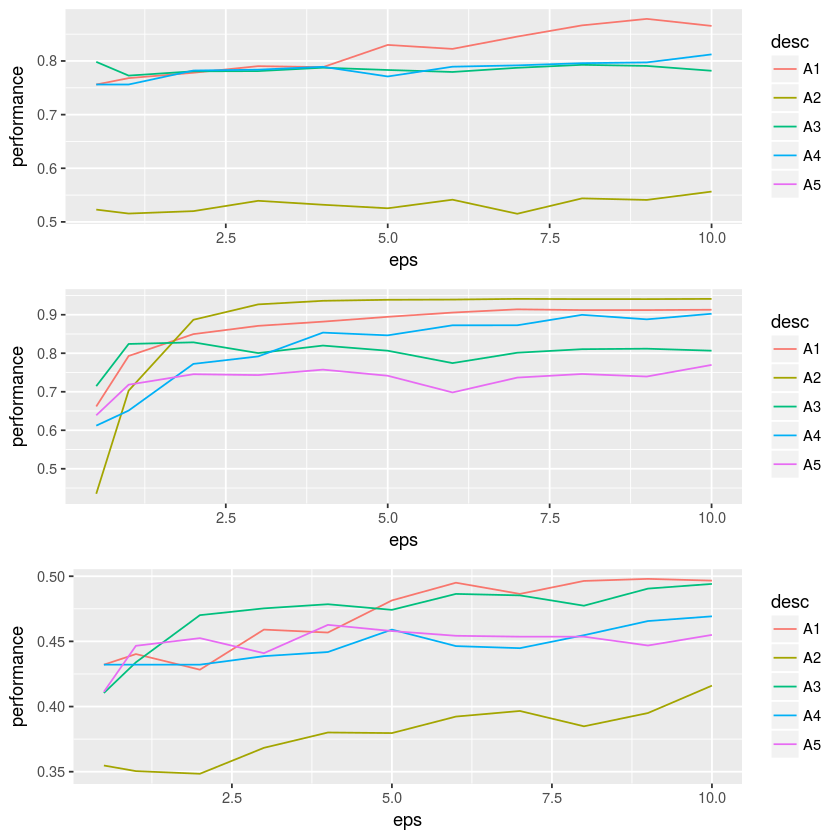
\includegraphics[scale=0.7]{Graph_Performances}
\end{center}
\caption{Performances of the five decision tree algorithms. The performance is measured from the prediction success rate on a validation set using a 30/70 validation to training split. Graph 1 does not have A5 because it takes such a long time to train, having a weak stopping criterion.}
\label{fig:datadep}
\end{figure}

In light of these experiments, we notice that stopping criteria, non-leaf-queries, and number of trees in the forest have a huge impact on the performance of the algorithm. What an analyst would really like to do is to shed light on these complicated relationships in an automated way. It would be easy for her to summarize all of the decision tree algorithms in a chart as in Figure \ref{alg:dtree}. Each of the two places where she is uncertain is marked with a label, L1 or L2. The goal of \Jostle{} is to learn automatically properties of the database that may lend to a certain decision at L1 or L2.

Our goal is to decide which heuristic is best
\begin{figure}
\begin{center}
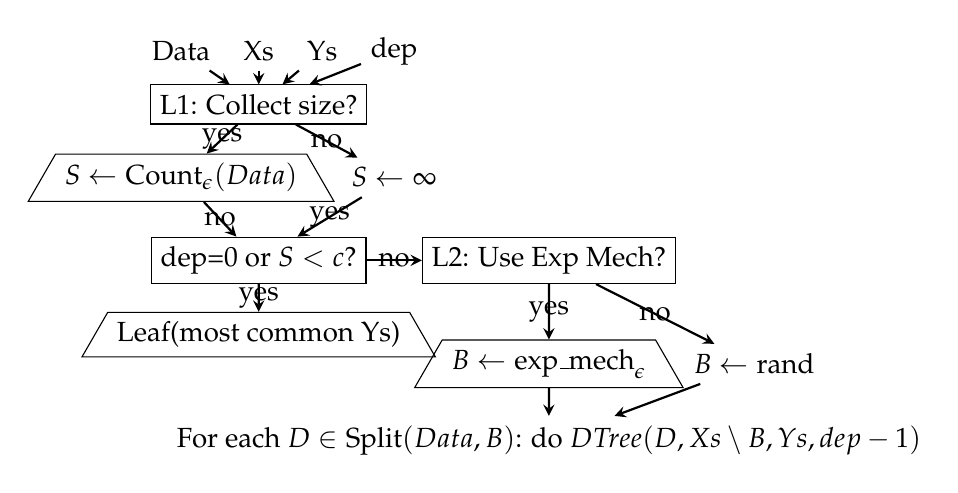
\begin{tikzpicture}[node distance=2cm]
\node (data_in) [io] {Data};
\node (xs_in) [io, right=0.5em of data_in] {Xs};
\node (ys_in) [io, right=0.5em of xs_in] {Ys};
\node (dep_in) [io, right=0.5em of ys_in] {dep};
\node (L1) [decision, below=0.5em of xs_in] {L1: Collect size?};
\draw [arrow] (data_in) -- (L1);
\draw [arrow] (xs_in) -- (L1);
\draw [arrow] (ys_in) -- (L1);
\draw [arrow] (dep_in) -- (L1);
\node (collect_yes) [process, below=3em of data_in] {$S \leftarrow \text{Count}_\epsilon(Data)$};
\node (collect_no) [io, below=3em of dep_in] {$S \leftarrow \infty$};
\draw [arrow] (L1) -- node {yes} (collect_yes);
\draw [arrow] (L1) -- node {no} (collect_no);
\node (stop) [decision, below=6em of xs_in] {dep=0 or $S < c$?};
\draw [arrow] (collect_no) -- node {yes} (stop);
\draw [arrow] (collect_yes) -- node {no} (stop);
\node (stop_yes) [process, below=1em of stop] {Leaf(most common Ys)};
\node (stop_no) [decision, right=2em of stop] {L2: Use Exp Mech?};
\draw [arrow] (stop) -- node {yes} (stop_yes);
\draw [arrow] (stop) -- node {no} (stop_no);
\node (exp_yes) [process, below=2em of stop_no] {$B \leftarrow \text{exp\_mech}_\epsilon$};
\node (exp_no) [io, right=0.5em of exp_yes] {$B \leftarrow \text{rand}$};
\draw [arrow] (stop_no) -- node {yes} (exp_yes);
\draw [arrow] (stop_no) -- node {no} (exp_no);
\node (wrap_up) [io, below=1em of exp_yes] {For each $D \in \text{Split}(Data, B)$: do $DTree(D, Xs\setminus B, Ys, dep-1)$};
\draw [arrow] (exp_yes) -- (wrap_up);
\draw [arrow] (exp_no) -- (wrap_up);
\end{tikzpicture}
\end{center}
\caption{Our decision tree algorithm with NoisyConditionals which learn the execution path from past histories. Depending on what the NoisyConditionals say, this algorithm is capable of expressing all the decision tree algorithms in \cite{Fletcher:2016}.}\label{alg:dtree}
\end{figure}
\bibliographystyle{plain}
\bibliography{Thesis}
\end{document}